% Polished Appendix A: Dataset Details (proofread by Claude). Original text is in main-original.tex.
\section{Technical Appendix: Dataset Details}
\label{app:dataset}
The figures and tables in this appendix come from earlier dataset releases and keep their original measurements and model renders, with labels translated into English. Each uses the versions and criteria of its own release and does not replace the integrated statistics or the main comparison.

\paragraph{Contact-based gravity screening.}
We model an 8\,mm stud spacing, a 9.6\,mm brick height, and a mass of 1\,g per occupied stud-brick cell. Each overlapping stud contributes four vertical contact points at the corners of a square with a half-width of 0.25 stud. The horizontal ground provides only compression, at the corners of ground-level brick footprints inset by 0.05 stud. A linear program (LP) seeks vertical force balance and balance of the two gravity-induced moments for every brick, and we verify the resulting contact forces against these equations. Once the final assembly passes, the same check is applied, from bottom to top, to the bricks up to each completed layer. Each stud-connected component of such a prefix is checked independently on the unanchored ground.

\paragraph{Tipping margin and clutch demand.}
The tipping margin is the minimum signed inward distance from the horizontal projection of the center of mass to the edges of the convex hull of the ground contacts. We convert the margin from studs to meters and reject zero or negative margins within numerical tolerance. If the compression-only LP is infeasible after this check, a second LP permits tension at internal stud contacts and minimizes the largest total tensile force over the four contact points of any single stud. We report this minimum required clutch force in newtons per stud; actual clutch capacity is not calibrated. A verified compression-only solution counts as a gravity-screening pass, while solutions that require tensile support are recorded separately.

\emph{Caption example.} The five captions of a model share a common prefix and add detail level by level. The L1 prompt is \textquotedblleft An oval birdhouse with curved roof, enclosed room and front entrance.\textquotedblright\ Its L5 description is: ``An oval birdhouse with curved roof, enclosed room and front entrance. The protective roof joins the walls; the circular front entrance reaches a real interior cavity. Curved substantial surfaces carry their continuously attached functional parts. Overall width is 1.15 times depth; height is 0.80 times width. Parts follow functional positions. Continuous red, tan, brown color regions distinguish the body and attachments. The front reveals functional parts; side and top views reveal depth, connections and layout.''

\begin{table}[!htbp]
\centering
\small
\setlength{\tabcolsep}{3pt}
\begin{tabular}{lrrr}
\toprule
Release & Passing & Added & Removed \\
\midrule
Strict v3 & 7,902 & -- & -- \\
Relaxed & 65,503 & 428,278 & 38,230 \\
Local refinement & 79,298 & 228,582 & 125 \\
\bottomrule
\end{tabular}
\caption{Geometric pass counts of the 80,000 source models under successive conversion releases, with the total voxels added and removed, as given in the corresponding release reports. The relaxed release allows several grounded components.}
\label{tab:conversion}
\end{table}

\begin{figure*}[!htbp]
\centering
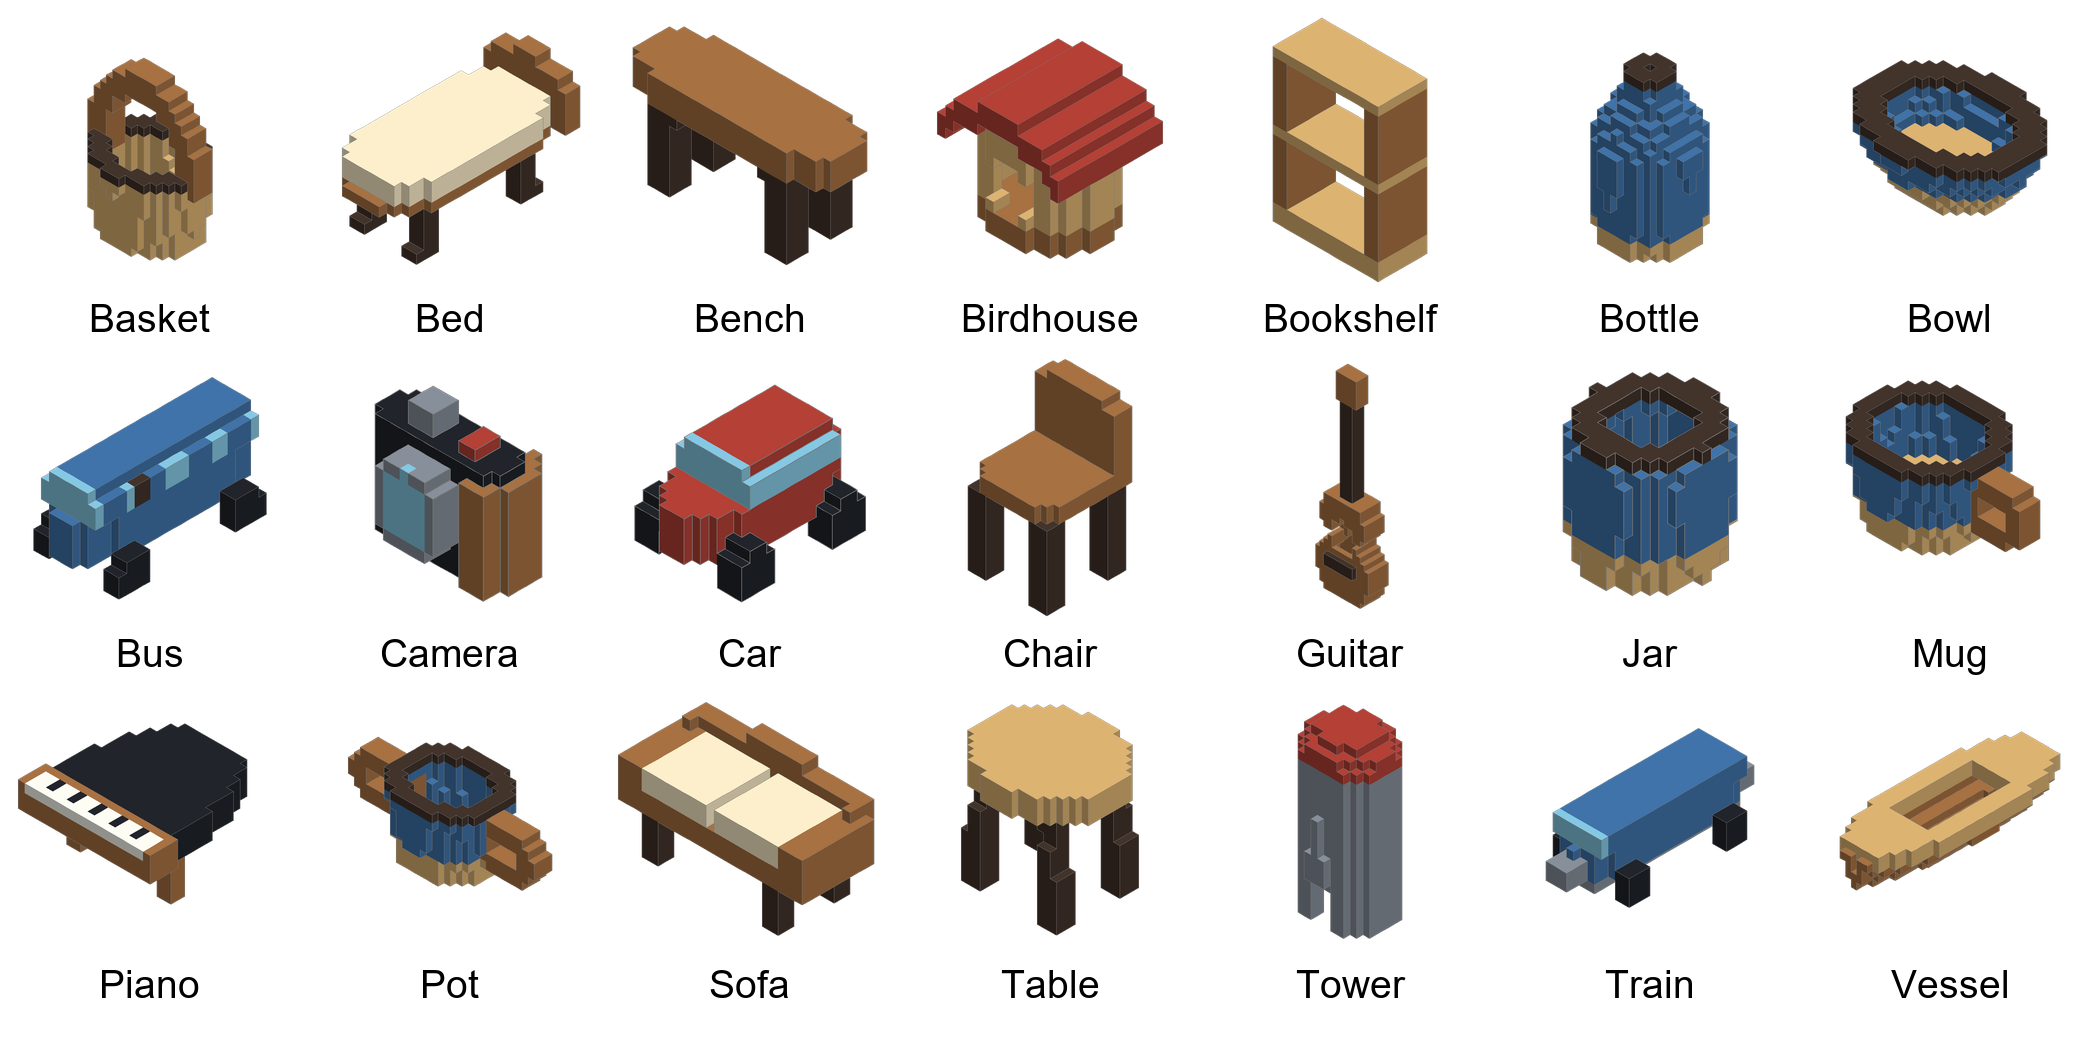
\includegraphics[width=\textwidth]{figures/image7_en.png}
\caption{Voxel model samples from the 21 object categories.}
\end{figure*}

\begin{figure*}[t]
\centering
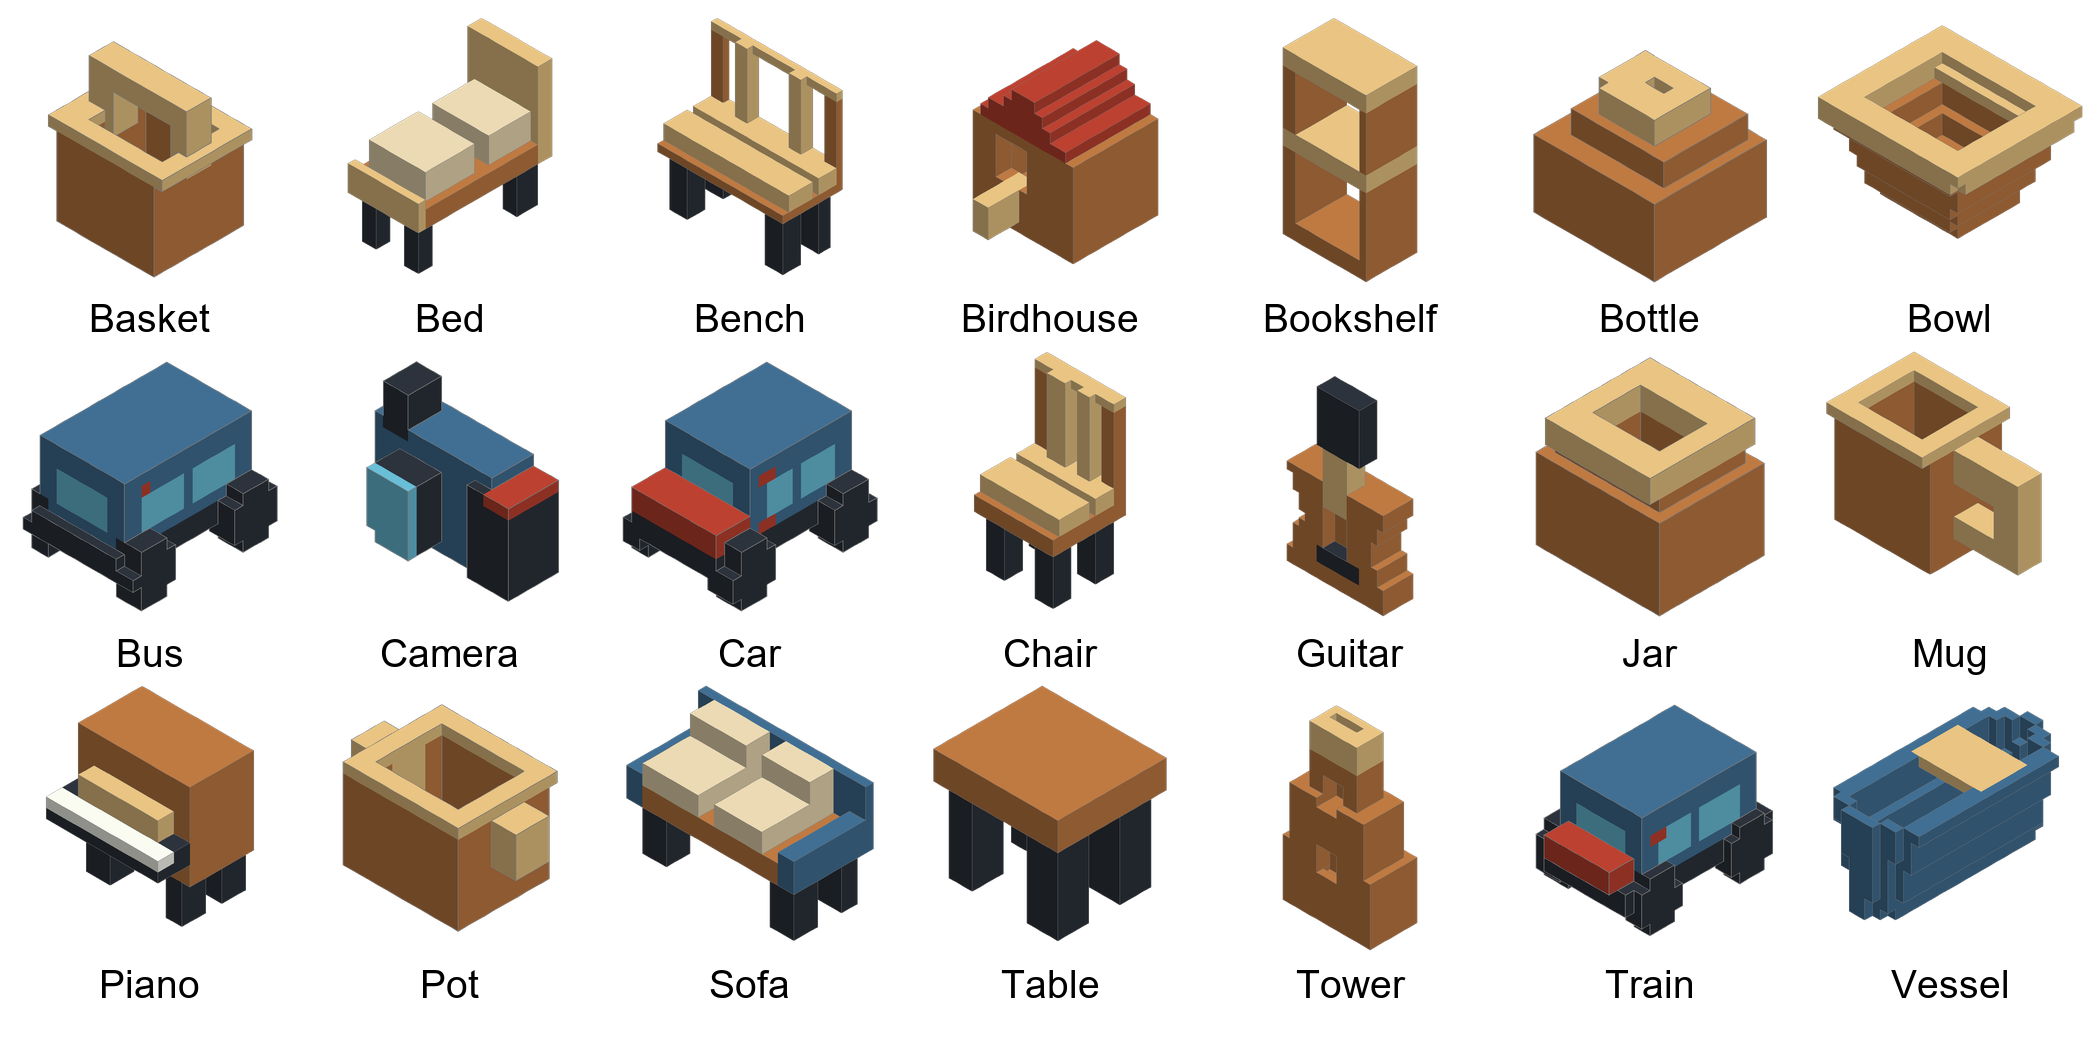
\includegraphics[width=\textwidth]{figures/image8_en.png}
\caption{Additional voxel model examples from an earlier release.}
\end{figure*}

\begin{figure*}[!htbp]
\centering
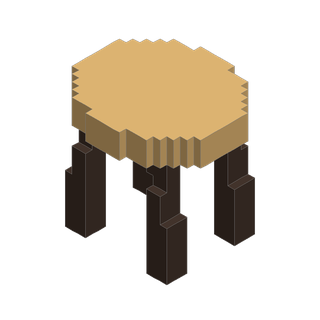
\includegraphics[width=0.118\textwidth]{figures/image4.png}\hfill
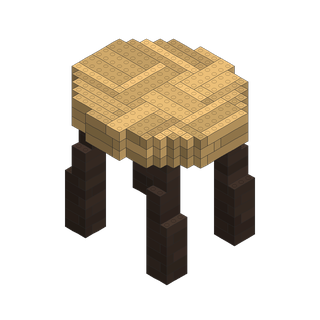
\includegraphics[width=0.118\textwidth]{figures/image5.png}\hfill
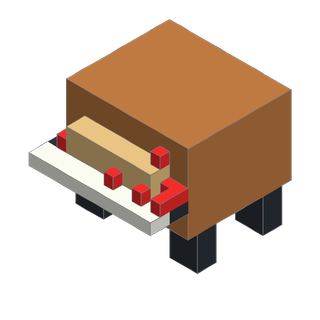
\includegraphics[width=0.118\textwidth]{figures/image2.png}\hfill
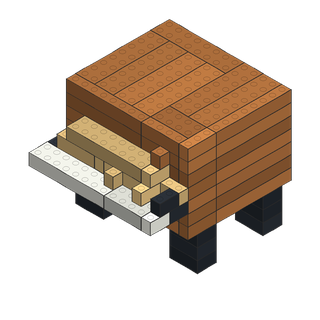
\includegraphics[width=0.118\textwidth]{figures/image3.png}\hfill
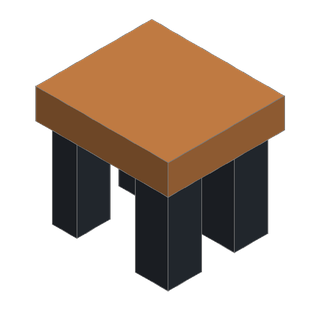
\includegraphics[width=0.118\textwidth]{figures/image9.png}\hfill
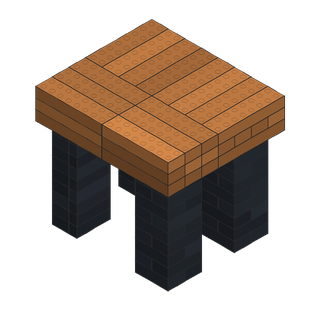
\includegraphics[width=0.118\textwidth]{figures/image10.png}\hfill

\includegraphics[width=0.118\textwidth]{figures/image11.png}\hfill
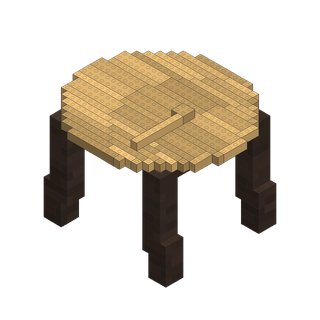
\includegraphics[width=0.118\textwidth]{figures/image12.png}
\caption{Examples of voxel targets and brick layouts after local repair, from an earlier release.}
\end{figure*}

\begin{figure*}[t]
\centering
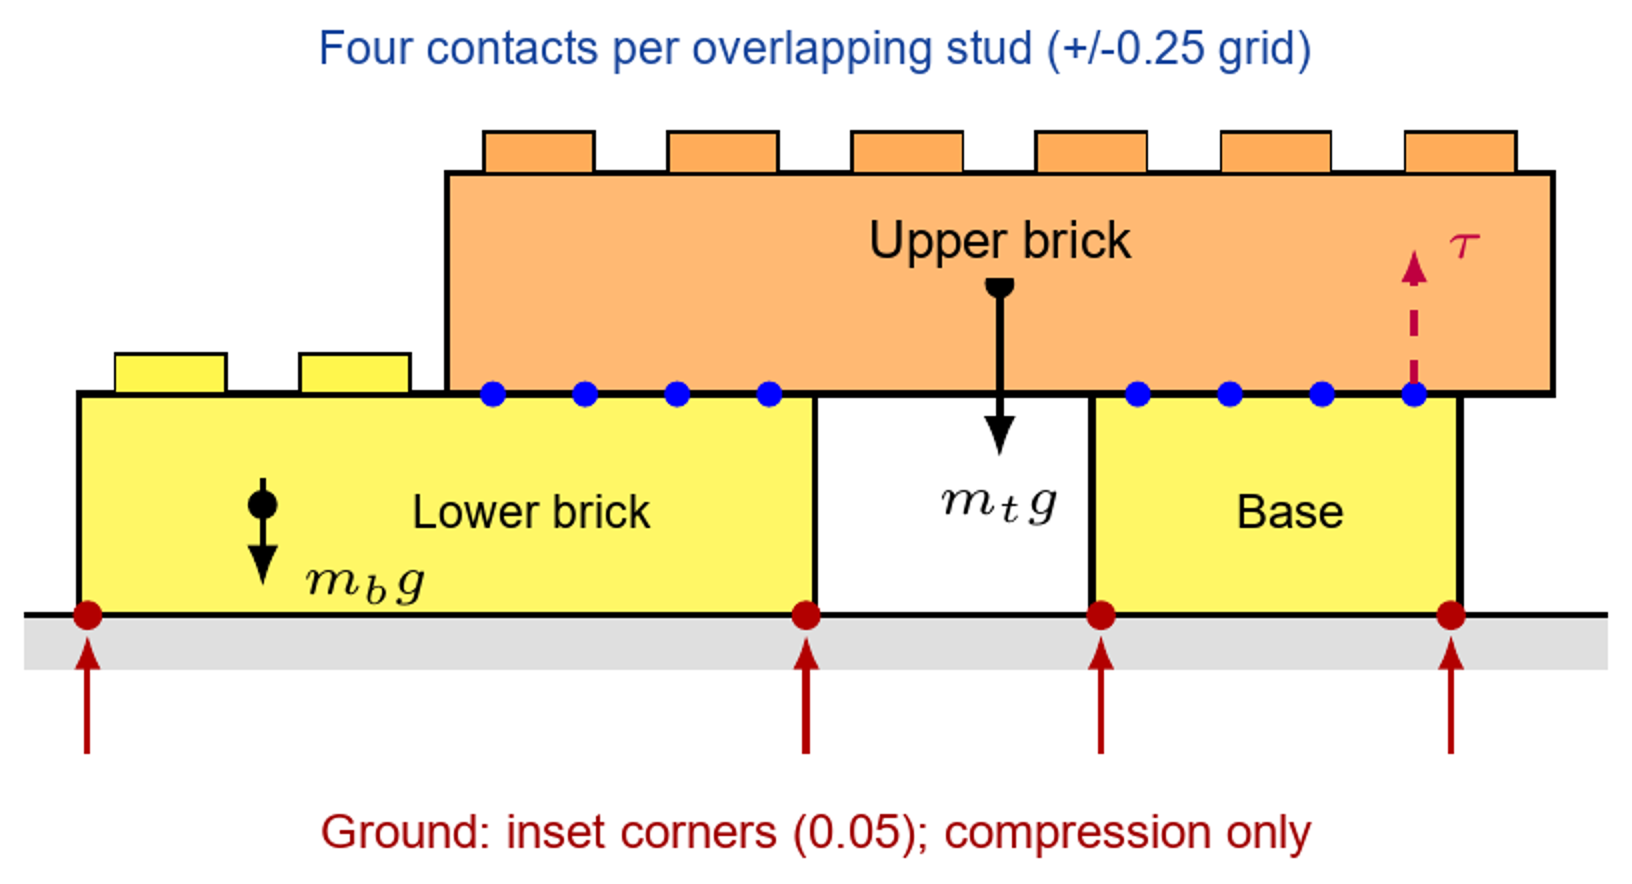
\includegraphics[width=0.75\textwidth]{figures/image13_en.png}
\caption{Contact-based gravity screening model from an earlier release, with English labels. The contact and ground assumptions are as stated above.}
\end{figure*}

\begin{figure*}[!htbp]
\centering
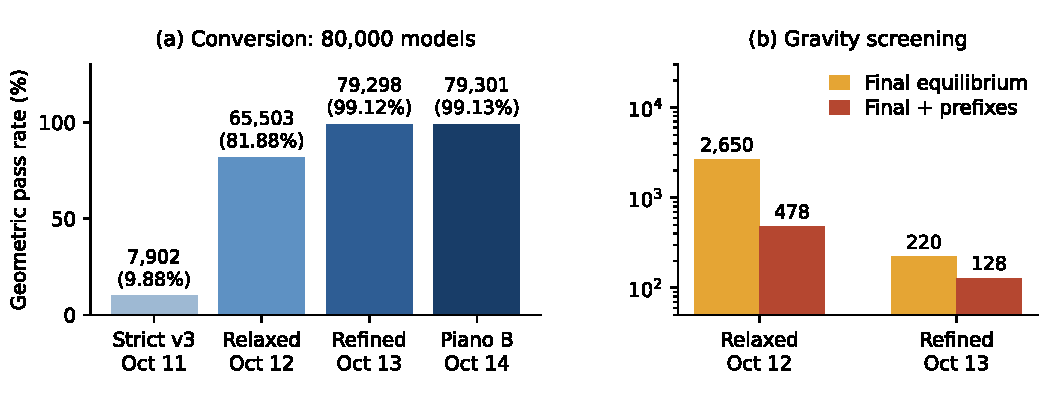
\includegraphics[width=\textwidth]{figures/image14_en.pdf}
\caption{Geometric conversion and screening outcomes across earlier releases; values as given in the corresponding release reports (Table~\ref{tab:conversion}).}
\end{figure*}

\begin{figure*}[!htbp]
\centering
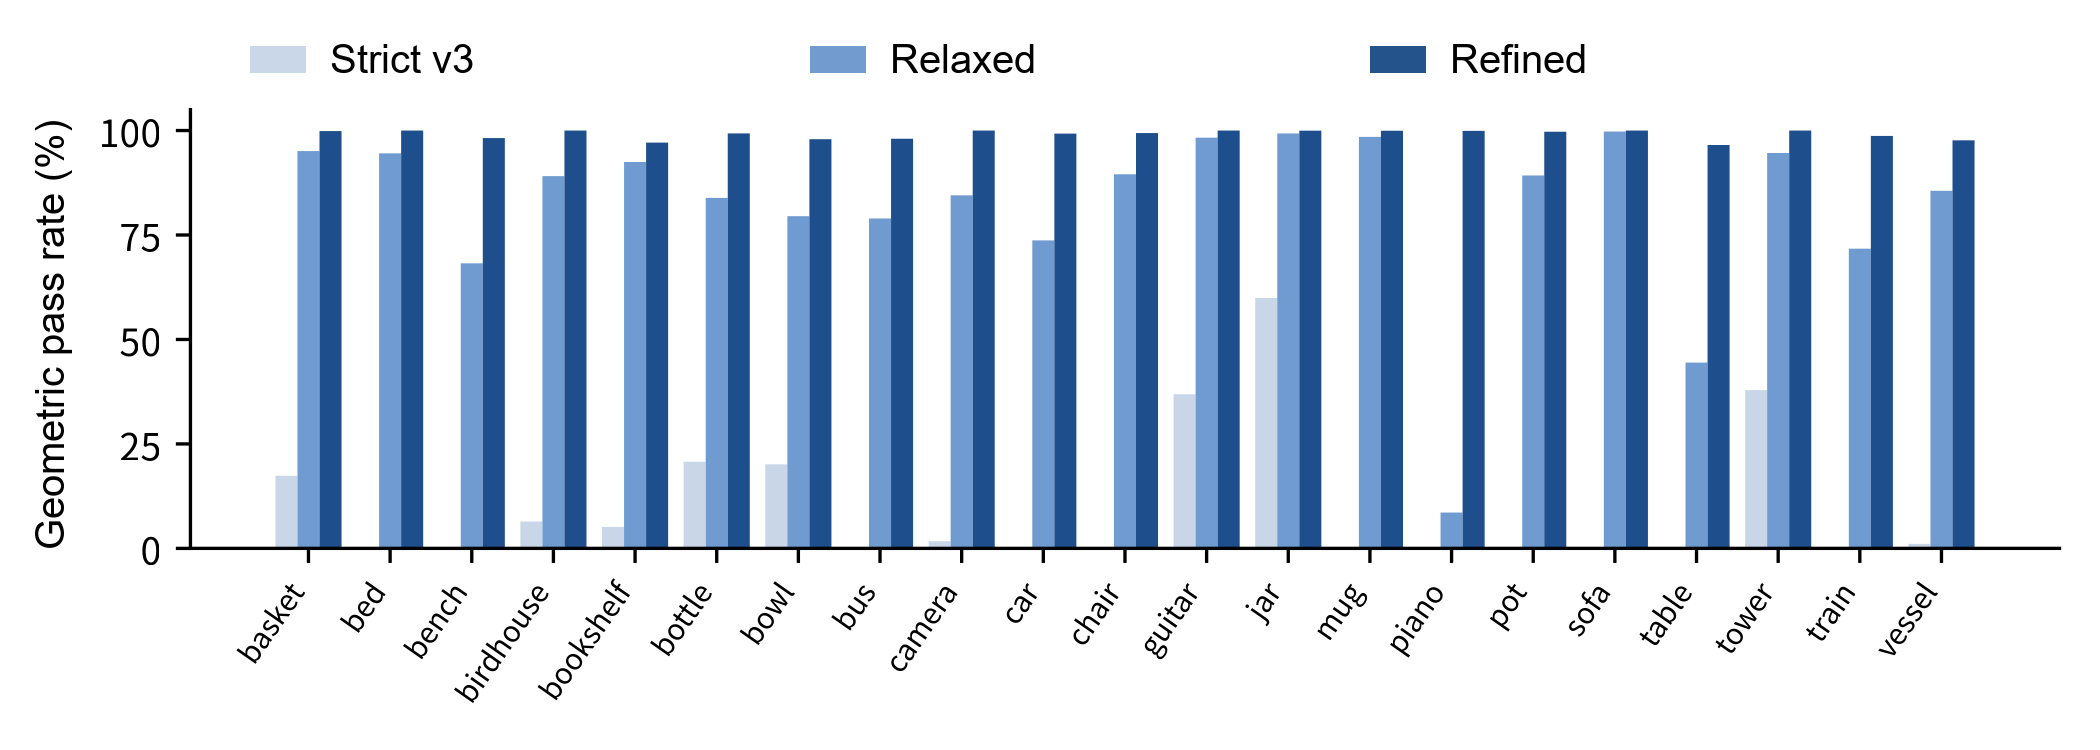
\includegraphics[width=\textwidth]{figures/image15_en.png}
\caption{Geometric pass rates by category for the three conversion releases in Table~\ref{tab:conversion}.}
\end{figure*}

\begin{figure*}[t]
\centering
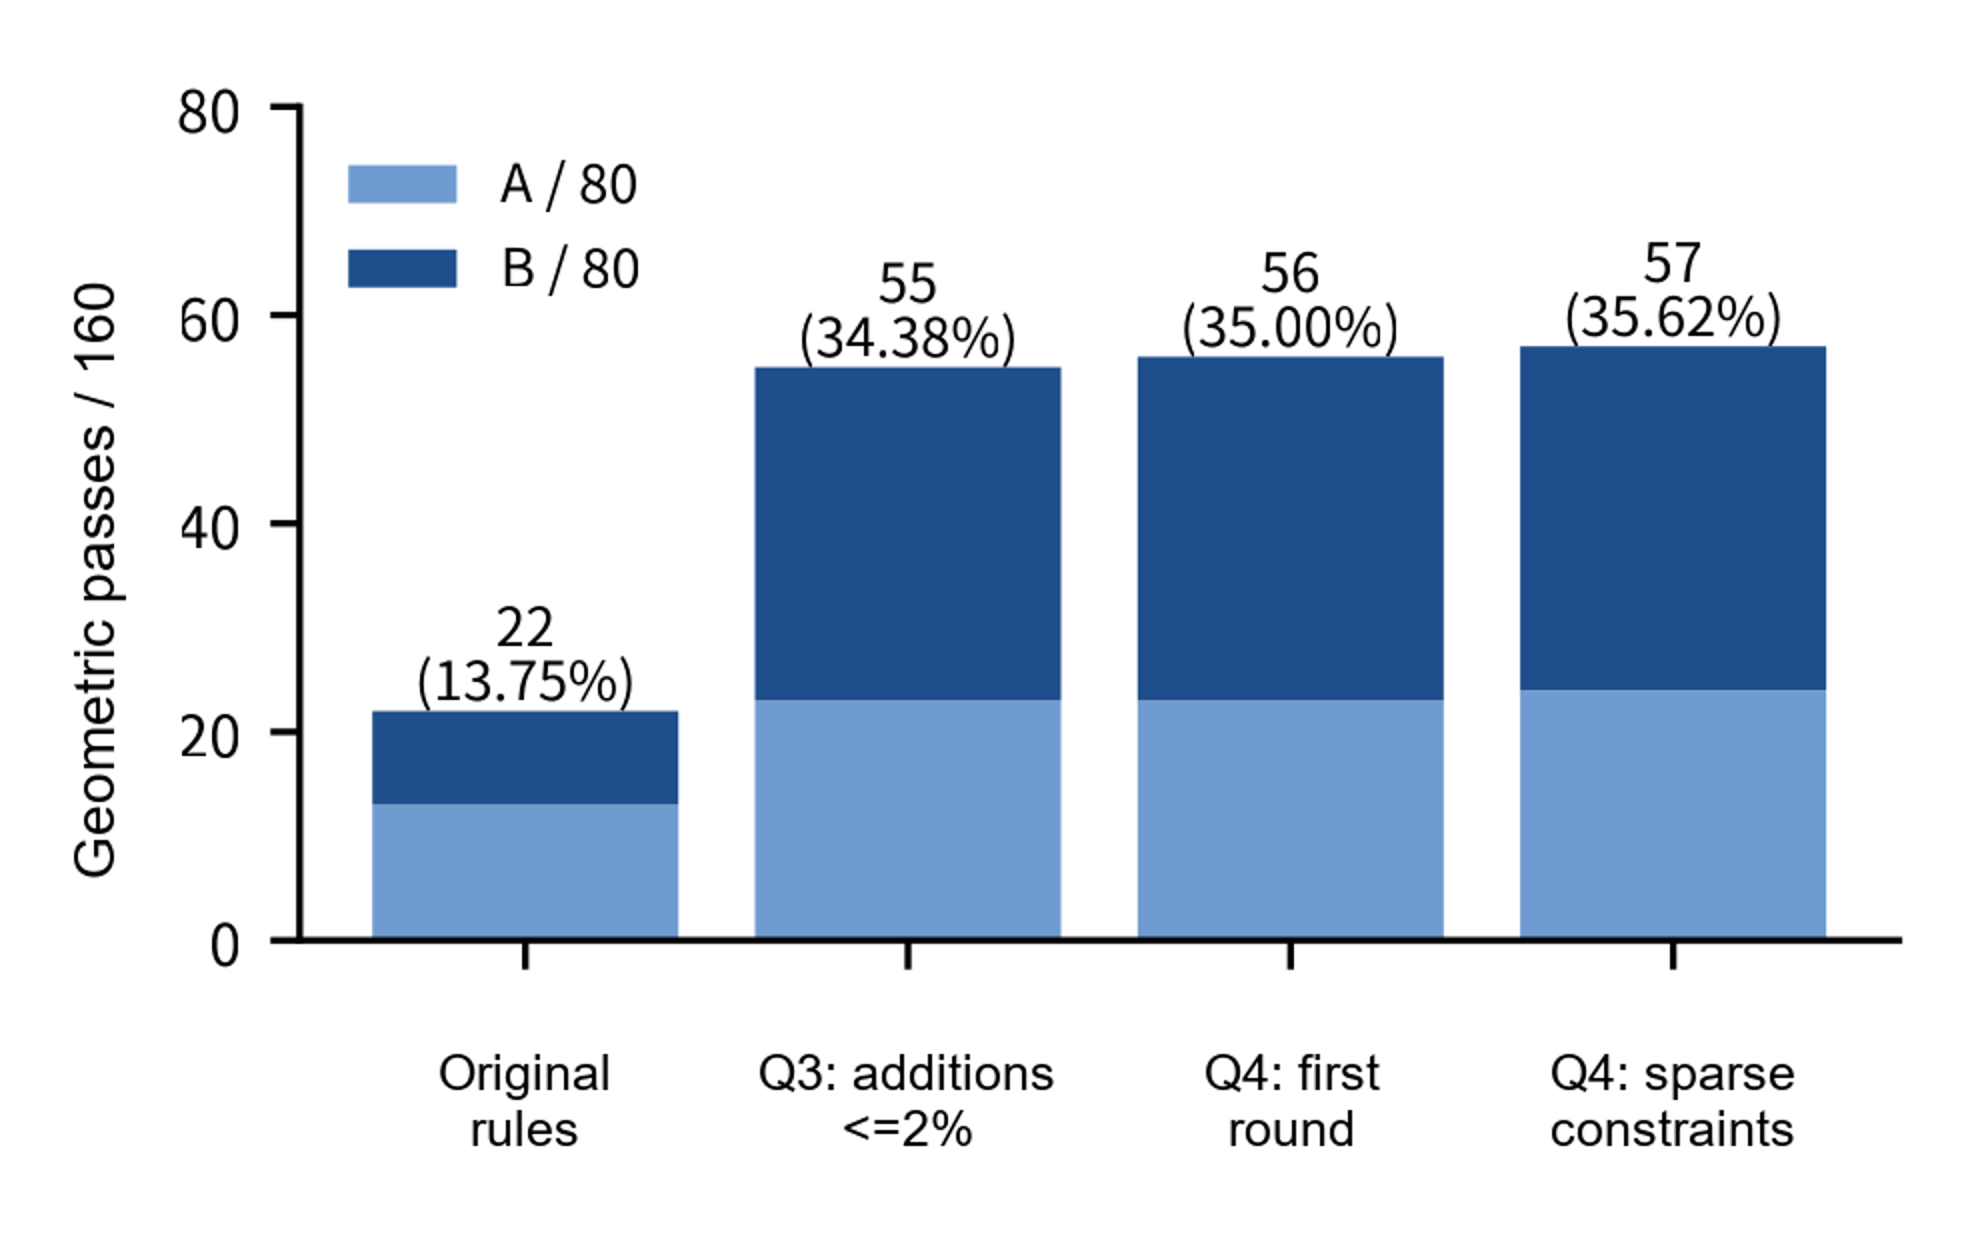
\includegraphics[width=0.72\textwidth]{figures/image16_en.png}
\caption{Geometric pass counts for the original rules, Q3, and two Q4 variants on the same 160-model sample (seed 38177). The Q4 rounds reuse this sample for tuning.}
\end{figure*}

\begin{figure*}[!htbp]
\centering
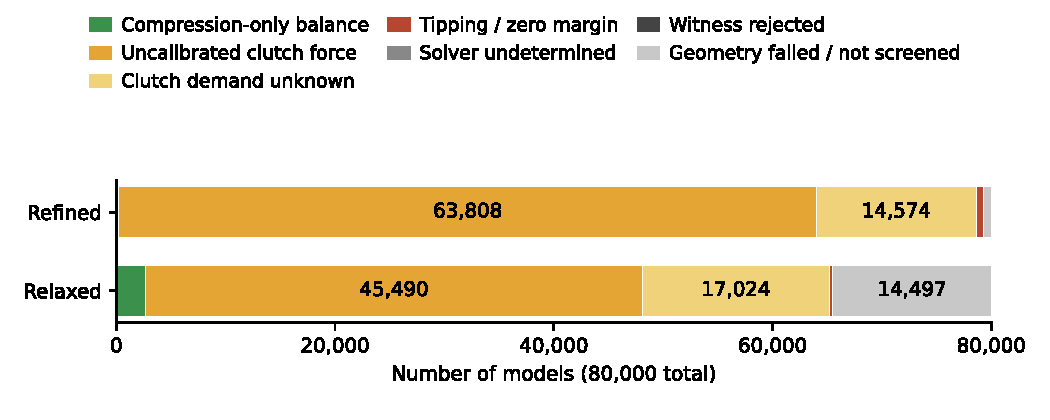
\includegraphics[width=\textwidth]{figures/image17_en.pdf}
\caption{Distributions of physical screening statuses in earlier releases; values as given in the corresponding release reports. Counts refer only to the releases shown and are reported separately from geometric pass rates.}
\end{figure*}
